% Options for packages loaded elsewhere
\PassOptionsToPackage{unicode}{hyperref}
\PassOptionsToPackage{hyphens}{url}
\PassOptionsToPackage{dvipsnames,svgnames,x11names}{xcolor}
%
\documentclass[
  letterpaper,
  DIV=11,
  numbers=noendperiod]{scrreprt}

\usepackage{amsmath,amssymb}
\usepackage{iftex}
\ifPDFTeX
  \usepackage[T1]{fontenc}
  \usepackage[utf8]{inputenc}
  \usepackage{textcomp} % provide euro and other symbols
\else % if luatex or xetex
  \usepackage{unicode-math}
  \defaultfontfeatures{Scale=MatchLowercase}
  \defaultfontfeatures[\rmfamily]{Ligatures=TeX,Scale=1}
\fi
\usepackage{lmodern}
\ifPDFTeX\else  
    % xetex/luatex font selection
\fi
% Use upquote if available, for straight quotes in verbatim environments
\IfFileExists{upquote.sty}{\usepackage{upquote}}{}
\IfFileExists{microtype.sty}{% use microtype if available
  \usepackage[]{microtype}
  \UseMicrotypeSet[protrusion]{basicmath} % disable protrusion for tt fonts
}{}
\makeatletter
\@ifundefined{KOMAClassName}{% if non-KOMA class
  \IfFileExists{parskip.sty}{%
    \usepackage{parskip}
  }{% else
    \setlength{\parindent}{0pt}
    \setlength{\parskip}{6pt plus 2pt minus 1pt}}
}{% if KOMA class
  \KOMAoptions{parskip=half}}
\makeatother
\usepackage{xcolor}
\setlength{\emergencystretch}{3em} % prevent overfull lines
\setcounter{secnumdepth}{5}
% Make \paragraph and \subparagraph free-standing
\makeatletter
\ifx\paragraph\undefined\else
  \let\oldparagraph\paragraph
  \renewcommand{\paragraph}{
    \@ifstar
      \xxxParagraphStar
      \xxxParagraphNoStar
  }
  \newcommand{\xxxParagraphStar}[1]{\oldparagraph*{#1}\mbox{}}
  \newcommand{\xxxParagraphNoStar}[1]{\oldparagraph{#1}\mbox{}}
\fi
\ifx\subparagraph\undefined\else
  \let\oldsubparagraph\subparagraph
  \renewcommand{\subparagraph}{
    \@ifstar
      \xxxSubParagraphStar
      \xxxSubParagraphNoStar
  }
  \newcommand{\xxxSubParagraphStar}[1]{\oldsubparagraph*{#1}\mbox{}}
  \newcommand{\xxxSubParagraphNoStar}[1]{\oldsubparagraph{#1}\mbox{}}
\fi
\makeatother

\usepackage{color}
\usepackage{fancyvrb}
\newcommand{\VerbBar}{|}
\newcommand{\VERB}{\Verb[commandchars=\\\{\}]}
\DefineVerbatimEnvironment{Highlighting}{Verbatim}{commandchars=\\\{\}}
% Add ',fontsize=\small' for more characters per line
\usepackage{framed}
\definecolor{shadecolor}{RGB}{241,243,245}
\newenvironment{Shaded}{\begin{snugshade}}{\end{snugshade}}
\newcommand{\AlertTok}[1]{\textcolor[rgb]{0.68,0.00,0.00}{#1}}
\newcommand{\AnnotationTok}[1]{\textcolor[rgb]{0.37,0.37,0.37}{#1}}
\newcommand{\AttributeTok}[1]{\textcolor[rgb]{0.40,0.45,0.13}{#1}}
\newcommand{\BaseNTok}[1]{\textcolor[rgb]{0.68,0.00,0.00}{#1}}
\newcommand{\BuiltInTok}[1]{\textcolor[rgb]{0.00,0.23,0.31}{#1}}
\newcommand{\CharTok}[1]{\textcolor[rgb]{0.13,0.47,0.30}{#1}}
\newcommand{\CommentTok}[1]{\textcolor[rgb]{0.37,0.37,0.37}{#1}}
\newcommand{\CommentVarTok}[1]{\textcolor[rgb]{0.37,0.37,0.37}{\textit{#1}}}
\newcommand{\ConstantTok}[1]{\textcolor[rgb]{0.56,0.35,0.01}{#1}}
\newcommand{\ControlFlowTok}[1]{\textcolor[rgb]{0.00,0.23,0.31}{\textbf{#1}}}
\newcommand{\DataTypeTok}[1]{\textcolor[rgb]{0.68,0.00,0.00}{#1}}
\newcommand{\DecValTok}[1]{\textcolor[rgb]{0.68,0.00,0.00}{#1}}
\newcommand{\DocumentationTok}[1]{\textcolor[rgb]{0.37,0.37,0.37}{\textit{#1}}}
\newcommand{\ErrorTok}[1]{\textcolor[rgb]{0.68,0.00,0.00}{#1}}
\newcommand{\ExtensionTok}[1]{\textcolor[rgb]{0.00,0.23,0.31}{#1}}
\newcommand{\FloatTok}[1]{\textcolor[rgb]{0.68,0.00,0.00}{#1}}
\newcommand{\FunctionTok}[1]{\textcolor[rgb]{0.28,0.35,0.67}{#1}}
\newcommand{\ImportTok}[1]{\textcolor[rgb]{0.00,0.46,0.62}{#1}}
\newcommand{\InformationTok}[1]{\textcolor[rgb]{0.37,0.37,0.37}{#1}}
\newcommand{\KeywordTok}[1]{\textcolor[rgb]{0.00,0.23,0.31}{\textbf{#1}}}
\newcommand{\NormalTok}[1]{\textcolor[rgb]{0.00,0.23,0.31}{#1}}
\newcommand{\OperatorTok}[1]{\textcolor[rgb]{0.37,0.37,0.37}{#1}}
\newcommand{\OtherTok}[1]{\textcolor[rgb]{0.00,0.23,0.31}{#1}}
\newcommand{\PreprocessorTok}[1]{\textcolor[rgb]{0.68,0.00,0.00}{#1}}
\newcommand{\RegionMarkerTok}[1]{\textcolor[rgb]{0.00,0.23,0.31}{#1}}
\newcommand{\SpecialCharTok}[1]{\textcolor[rgb]{0.37,0.37,0.37}{#1}}
\newcommand{\SpecialStringTok}[1]{\textcolor[rgb]{0.13,0.47,0.30}{#1}}
\newcommand{\StringTok}[1]{\textcolor[rgb]{0.13,0.47,0.30}{#1}}
\newcommand{\VariableTok}[1]{\textcolor[rgb]{0.07,0.07,0.07}{#1}}
\newcommand{\VerbatimStringTok}[1]{\textcolor[rgb]{0.13,0.47,0.30}{#1}}
\newcommand{\WarningTok}[1]{\textcolor[rgb]{0.37,0.37,0.37}{\textit{#1}}}

\providecommand{\tightlist}{%
  \setlength{\itemsep}{0pt}\setlength{\parskip}{0pt}}\usepackage{longtable,booktabs,array}
\usepackage{calc} % for calculating minipage widths
% Correct order of tables after \paragraph or \subparagraph
\usepackage{etoolbox}
\makeatletter
\patchcmd\longtable{\par}{\if@noskipsec\mbox{}\fi\par}{}{}
\makeatother
% Allow footnotes in longtable head/foot
\IfFileExists{footnotehyper.sty}{\usepackage{footnotehyper}}{\usepackage{footnote}}
\makesavenoteenv{longtable}
\usepackage{graphicx}
\makeatletter
\newsavebox\pandoc@box
\newcommand*\pandocbounded[1]{% scales image to fit in text height/width
  \sbox\pandoc@box{#1}%
  \Gscale@div\@tempa{\textheight}{\dimexpr\ht\pandoc@box+\dp\pandoc@box\relax}%
  \Gscale@div\@tempb{\linewidth}{\wd\pandoc@box}%
  \ifdim\@tempb\p@<\@tempa\p@\let\@tempa\@tempb\fi% select the smaller of both
  \ifdim\@tempa\p@<\p@\scalebox{\@tempa}{\usebox\pandoc@box}%
  \else\usebox{\pandoc@box}%
  \fi%
}
% Set default figure placement to htbp
\def\fps@figure{htbp}
\makeatother
% definitions for citeproc citations
\NewDocumentCommand\citeproctext{}{}
\NewDocumentCommand\citeproc{mm}{%
  \begingroup\def\citeproctext{#2}\cite{#1}\endgroup}
\makeatletter
 % allow citations to break across lines
 \let\@cite@ofmt\@firstofone
 % avoid brackets around text for \cite:
 \def\@biblabel#1{}
 \def\@cite#1#2{{#1\if@tempswa , #2\fi}}
\makeatother
\newlength{\cslhangindent}
\setlength{\cslhangindent}{1.5em}
\newlength{\csllabelwidth}
\setlength{\csllabelwidth}{3em}
\newenvironment{CSLReferences}[2] % #1 hanging-indent, #2 entry-spacing
 {\begin{list}{}{%
  \setlength{\itemindent}{0pt}
  \setlength{\leftmargin}{0pt}
  \setlength{\parsep}{0pt}
  % turn on hanging indent if param 1 is 1
  \ifodd #1
   \setlength{\leftmargin}{\cslhangindent}
   \setlength{\itemindent}{-1\cslhangindent}
  \fi
  % set entry spacing
  \setlength{\itemsep}{#2\baselineskip}}}
 {\end{list}}
\usepackage{calc}
\newcommand{\CSLBlock}[1]{\hfill\break\parbox[t]{\linewidth}{\strut\ignorespaces#1\strut}}
\newcommand{\CSLLeftMargin}[1]{\parbox[t]{\csllabelwidth}{\strut#1\strut}}
\newcommand{\CSLRightInline}[1]{\parbox[t]{\linewidth - \csllabelwidth}{\strut#1\strut}}
\newcommand{\CSLIndent}[1]{\hspace{\cslhangindent}#1}

\KOMAoption{captions}{tableheading}
\makeatletter
\@ifpackageloaded{bookmark}{}{\usepackage{bookmark}}
\makeatother
\makeatletter
\@ifpackageloaded{caption}{}{\usepackage{caption}}
\AtBeginDocument{%
\ifdefined\contentsname
  \renewcommand*\contentsname{Table of contents}
\else
  \newcommand\contentsname{Table of contents}
\fi
\ifdefined\listfigurename
  \renewcommand*\listfigurename{List of Figures}
\else
  \newcommand\listfigurename{List of Figures}
\fi
\ifdefined\listtablename
  \renewcommand*\listtablename{List of Tables}
\else
  \newcommand\listtablename{List of Tables}
\fi
\ifdefined\figurename
  \renewcommand*\figurename{Figure}
\else
  \newcommand\figurename{Figure}
\fi
\ifdefined\tablename
  \renewcommand*\tablename{Table}
\else
  \newcommand\tablename{Table}
\fi
}
\@ifpackageloaded{float}{}{\usepackage{float}}
\floatstyle{ruled}
\@ifundefined{c@chapter}{\newfloat{codelisting}{h}{lop}}{\newfloat{codelisting}{h}{lop}[chapter]}
\floatname{codelisting}{Listing}
\newcommand*\listoflistings{\listof{codelisting}{List of Listings}}
\makeatother
\makeatletter
\makeatother
\makeatletter
\@ifpackageloaded{caption}{}{\usepackage{caption}}
\@ifpackageloaded{subcaption}{}{\usepackage{subcaption}}
\makeatother

\usepackage{bookmark}

\IfFileExists{xurl.sty}{\usepackage{xurl}}{} % add URL line breaks if available
\urlstyle{same} % disable monospaced font for URLs
\hypersetup{
  pdftitle={Learning-Diary1},
  pdfauthor={Luo Huangchen},
  colorlinks=true,
  linkcolor={blue},
  filecolor={Maroon},
  citecolor={Blue},
  urlcolor={Blue},
  pdfcreator={LaTeX via pandoc}}


\title{Learning-Diary1}
\author{Luo Huangchen}
\date{2025-03-18}

\begin{document}
\maketitle

\renewcommand*\contentsname{Table of contents}
{
\hypersetup{linkcolor=}
\setcounter{tocdepth}{2}
\tableofcontents
}

\bookmarksetup{startatroot}

\chapter*{Welcome!}\label{welcome}
\addcontentsline{toc}{chapter}{Welcome!}

\markboth{Welcome!}{Welcome!}

Hi everyone! I'm Luo Huangchen, currently pursuing a master's degree in
Urban Spatial Science, with a focus on transportation planning, spatial
data analysis, and remote sensing applications. I enjoy using data to
tell stories and exploring new technologies to make cities smarter and
more livable. During my undergraduate years, I participated in various
projects related to smart transportation, sustainable urban development,
and traffic system optimization. I've worked extensively with tools like
ArcGIS, Python, and R for data analysis. Recently, I've been researching
mangrove and wetland conservation in the Greater Bay Area using remote
sensing, which has been both challenging and exciting! Beyond academics,
I love traveling, photography, and trying new things. I often optimize
SQL queries, simulate traffic flows with VISSIM, and conduct spatial
analyses with GIS. Of course, I also take some time to relax by watching
shows and unwinding. 😆 I'm looking forward to connecting with
like-minded people and exploring the fascinating world of cities
together! I'm really passionate about remote sensing, and I'm excited to
learn and gain more knowledge in CASA0023. I'm looking forward to all
the lectures and workshops!

\begin{verbatim}

`<!-- quarto-file-metadata: eyJyZXNvdXJjZURpciI6Ii4ifQ== -->`{=html}

```{=html}
<!-- quarto-file-metadata: eyJyZXNvdXJjZURpciI6Ii4iLCJib29rSXRlbVR5cGUiOiJjaGFwdGVyIiwiYm9va0l0ZW1OdW1iZXIiOjEsImJvb2tJdGVtRmlsZSI6IldlZWsxLnFtZCIsImJvb2tJdGVtRGVwdGgiOjB9 -->
\end{verbatim}

\bookmarksetup{startatroot}

\chapter*{Week 1 Learning Diary}\label{week-1-learning-diary}
\addcontentsline{toc}{chapter}{Week 1 Learning Diary}

\markboth{Week 1 Learning Diary}{Week 1 Learning Diary}

\bookmarksetup{startatroot}

\chapter*{🌍 Week1}\label{week1}
\addcontentsline{toc}{chapter}{🌍 Week1}

\markboth{🌍 Week1}{🌍 Week1}

\section*{Summary}\label{summary}
\addcontentsline{toc}{section}{Summary}

\markright{Summary}

This week's course introduces the basic concepts and methods of remote
sensing (Remote Sensing). Remote sensing refers to the technology of
obtaining information about the Earth from a distance, usually with the
help of sensors on platforms such as satellites, aircraft or drones
(\textbf{Campbell2011?}). We discussed in depth the difference between
active and passive remote sensing: active remote sensing uses signals
emitted by itself (e.g.~radar, lidar, etc.) and receives reflected
information, while passive remote sensing relies on information
reflected from sunlight hitting the surface, such as the Landsat and
Sentinel satellites (\textbf{Jensen2009?}).

Remote sensing data usually have four types of resolution: spatial
resolution (pixel size), spectral resolution (number of detected bands),
temporal resolution (revisit period) and radiometric resolution
(sensitivity of detected spectra). These resolutions determine the
application range and accuracy of remote sensing data. At the same time,
the electromagnetic spectral signature (Spectral Signature) of the
Earth's surface enables remote sensing technology to effectively
differentiate between different feature types, such as vegetation, water
bodies, and soils. In addition, we discussed that the acquisition of
remote sensing data may be affected by atmospheric conditions such as
clouds and haze, which makes it necessary to ensure the quality and
validity of data through atmospheric correction and other means
(\textbf{Schowengerdt2007?}).

\section*{Applications}\label{applications}
\addcontentsline{toc}{section}{Applications}

\markright{Applications}

Remote sensing technology has in fact long permeated every aspect of our
lives, especially in the matter of responding to natural disasters,
where its role is becoming increasingly important. For example, the
synthetic aperture radar (SAR) in active remote sensing, which we
mentioned in class, is particularly powerful in flood detection.
Traditional optical satellites are easily blocked by clouds, but SAR is
different, it can `penetrate' the clouds to monitor the ground
conditions around the clock, so it is particularly useful in emergency
situations such as floods (Amitrano \emph{et al.}, 2024). A recent
reading also highlights that with climate change and increased
urbanisation, flooding is becoming more frequent, making it vital to be
able to identify and monitor flooded areas quickly and effectively, a
need that SAR data meets, and one that can help governments to respond
quickly and allocate resources for disaster relief(\textbf{twele2016?}).

\begin{figure}[H]

{\centering 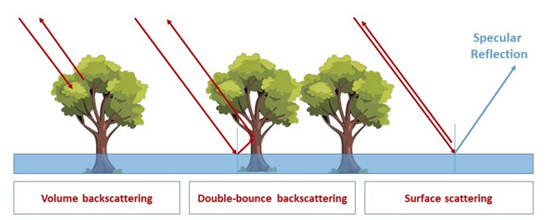
\includegraphics[width=0.7\linewidth,height=\textheight,keepaspectratio]{images/flood.png}

}

\caption{Fig. 1 Three types of scattering of radar signals}

\end{figure}%

\emph{Source: \href{https://doi.org/10.3390/rs16040656}{Amitrano et
al.~(2024)}}

In addition to flood monitoring, passive remote sensing data are also
widely used, such as the Landsat and Sentinel-2 satellites that we often
hear about, and their applications in agriculture and the ecological
environment are particularly numerous. As an example, satellite data can
be used to calculate the vegetation index (NDVI), which helps the
agricultural sector to more accurately assess the growth of crops and
predict yields, and can even monitor changes in the ecological
environment in real time. Moreover, using cloud computing platforms such
as Google Earth Engine, people can easily analyse large-scale land cover
changes and even monitor global ecological trends (Zhu and Woodcock,
2014; Gorelick \emph{et al.}, 2017).

\begin{figure}[H]

{\centering 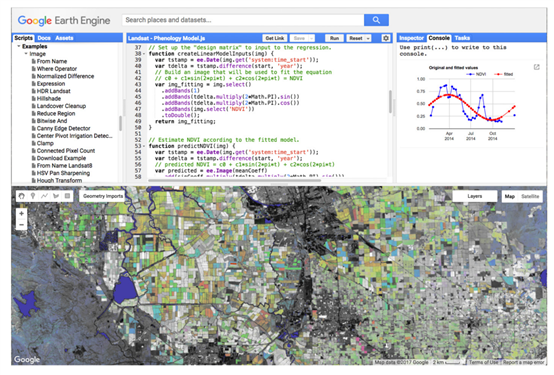
\includegraphics[width=0.7\linewidth,height=\textheight,keepaspectratio]{images/Geewk1.png}

}

\caption{Figure 2 Schematic of the Google Earth Engine}

\end{figure}%

\emph{Source: \href{https://doi.org/10.1016/j.rse.2017.06.031}{Gorelick
et al.~(2017)}}

However, remote sensing is not a panacea, especially in cities and areas
with vegetation cover, where SAR data can still be difficult to analyse.
This is because buildings and vegetation in cities can cause complex
signal reflections, making accurate identification of flooded areas
tricky at times. Overall, however, the convenience and comprehensiveness
provided by remote sensing data gives us more initiative in disaster
response and environmental management, and the future development
prospects are still worth looking forward to.

\section*{Reflection}\label{reflection}
\addcontentsline{toc}{section}{Reflection}

\markright{Reflection}

The first week of remote sensing class made me realise right away that
this technology is not just an abstract theory in the academic field,
but a real tool that can make a difference in people's lives. Of
interest to me was the fact that active remote sensing (SAR), which we
mentioned in class, has particularly prominent applications in natural
disaster, especially flood monitoring. My previous understanding of
remote sensing may have been limited to the simple application of
satellite imagery, but I had no idea that it also has such great
potential to address the risks associated with urbanisation and to
protect people's lives and property.

At the same time, I also noticed that although SAR can overcome the
shortcomings of traditional optical images (such as the influence of
cloud cover), there are still some challenges in its practical
application. For example, the processing of SAR data in complex
environments such as cities is still difficult, which reminds me that
there are still quite a few practical problems to overcome between the
development of the technology and the landing of the application. In
addition, I am particularly interested in cloud platforms such as Google
Earth Engine, which greatly reduces the threshold of remote sensing data
analysis and allows us to quickly carry out large-scale environmental
monitoring on a global scale, which is very attractive for both academic
research and practical work.

One of the deepest feelings I got from this class is that remote sensing
technology has really brought people closer to the Earth's environment.
Although there are still a lot of technical details that I need to learn
in depth, I am already looking forward to what I can learn next and the
role this knowledge can play in my future studies and career.

\bookmarksetup{startatroot}

\chapter{Week 2 Learning Diary}\label{week-2-learning-diary}

\section{Week2}\label{week2}

📢 Week 2: Creating PPTs with xaringan This week, we will be using
xaringan, an R Markdown package, to create slides. xaringan allows us to
build flexible, interactive, and beautifully styled presentations using
simple Markdown syntax. It's a powerful tool for sharing research
findings, data visualizations, and spatial analysis results in a
professional and customizable way.

Throughout this week, we will explore how to: ✅ Set up a basic xaringan
presentation ✅ Customize themes and layouts ✅ Integrate code, plots,
and interactive elements

I'm excited to dive into this and see how we can make engaging
presentations with xaringan! 🚀

\bookmarksetup{startatroot}

\chapter{Week 3 Learning Diary}\label{week-3-learning-diary}

\section{📢 Week 3: Learning
Corrections}\label{week-3-learning-corrections}

\section{Summary}\label{summary-1}

This week's course took us on an in-depth exploration of important data
correction methods and technical background in remote sensing data
processing. First, we reviewed the history of the famous
\textbf{Landsat} series of satellite data, with a special focus on the
key contributions of technician Virginia Norwood, whose design of the
digital multispectral scanner (\emph{Multispectral Scanner} (MSS))
replaced the traditional analogue camera technique and drove a major
change in remote sensing technology. Today, Norwood's \emph{Whisk broom}
scanning technique is at the heart of remote sensing data acquisition.

In terms of data processing, we specifically learnt about three key
methods, namely geometric correction, atmospheric correction and
orthometric correction. Geometric correction addresses the spatial error
between the satellite image and the actual geographic location by
calibrating the image position through Ground Control Points (GCPs).
Atmospheric correction deals with the data bias caused by the
atmosphere, including relative correction (e.g.~dark object subtraction,
pseudo-invariant feature method) and absolute correction (e.g.~FLAASH
model) to ensure that the acquired data reflect the surface conditions
more realistically. Orthometric corrections are used to correct image
distortions caused by the angle of observation of the satellite, using
mathematical models and surface elevation data to produce an accurate
image as if viewed from directly above.

\subsection{Summary of Remote Sensing Data Corrections}

\begin{longtable}[]{@{}
  >{\raggedright\arraybackslash}p{(\linewidth - 4\tabcolsep) * \real{0.1340}}
  >{\raggedright\arraybackslash}p{(\linewidth - 4\tabcolsep) * \real{0.2823}}
  >{\raggedright\arraybackslash}p{(\linewidth - 4\tabcolsep) * \real{0.5837}}@{}}
\toprule\noalign{}
\begin{minipage}[b]{\linewidth}\raggedright
\textbf{Correction Method}
\end{minipage} & \begin{minipage}[b]{\linewidth}\raggedright
\textbf{Main Purpose}
\end{minipage} & \begin{minipage}[b]{\linewidth}\raggedright
\textbf{Common Techniques}
\end{minipage} \\
\midrule\noalign{}
\endhead
\bottomrule\noalign{}
\endlastfoot
\textbf{Geometric Correction} & Ensures spatial accuracy of images &
Ground Control Points (GCP) \\
\textbf{Atmospheric Correction} & Removes atmospheric interference
(clouds, haze, etc.) & - Relative Correction: Dark Object Subtraction,
Pseudo-Invariant Feature Method - Absolute Correction: FLAASH Model \\
\textbf{Orthorectification} & Eliminates distortions caused by satellite
viewing angles & Mathematical models, DEM-based corrections \\
\end{longtable}

\begin{verbatim}
                
\end{verbatim}

Through this week's study, I have gained a deep understanding of the
complexity behind the process of remote sensing data processing, the
seemingly tedious but very important steps that ensure the efficiency
and accuracy of the data in scientific research and practical
applications, and enable us to use remote sensing data more confidently
in analyses and decision-making.

\section{Application}\label{application}

After studying the remote sensing data correction techniques during the
week, I purposely reviewed some examples of remote sensing correction
applications in practical research, which helped me better understand
the practical value of these methods. For example, in crop estimation
studies, atmospheric correction techniques have a significant impact on
the accuracy of vegetation indices. The accuracy of NDVI data can be
significantly improved by accurate atmospheric correction, which can
better monitor the true health of crops and thus help farmers to
increase yields and reduce losses (Song \emph{et al.} (2001)). In
addition, some studies have also clearly pointed out that remote sensing
data without correct geometric correction may lead to significant
overestimation or underestimation of forest fire area (Roy \emph{et al.}
(2016)). Therefore, the importance of accurate geometric correction in
the field of disaster management cannot be overstated.

The application of orthometric correction, on the other hand, reminds me
of practical examples in urban planning. For example, in urban expansion
studies, image distortion caused by satellite image tilting can
seriously affect the accurate measurement of urban area, which can be
effectively avoided after accurate ortho-correction, helping decision
makers to grasp urban expansion trends more accurately (Lefebvre,
Sannier and Corpetti (2016)). This study used Sentinel-2 data to update
the Copernicus High Resolution Impermeable Layer (HRL IMD), which
improves the accuracy of urban change monitoring through remote sensing
data fusion, as exemplified in the figure below which detects the
changes in the city of Rennes for the years 2012-2015. This shows that
orthorectification is not only applicable to traditional geographic
studies, but also plays a crucial role in modern large-scale urban
monitoring missions.

\begin{figure}[H]

{\centering 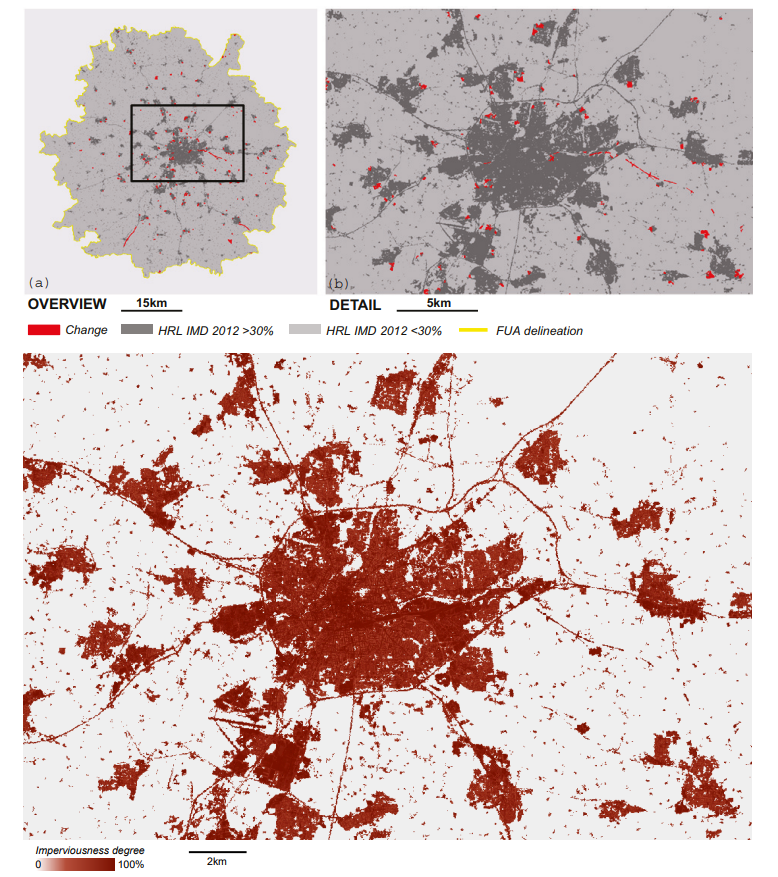
\includegraphics[width=0.8\linewidth,height=\textheight,keepaspectratio]{images/urban_change_rennes.png}

}

\caption{\textbf{Urban Change Detection in Rennes
(2012-2015)}\emph{\hfill\break
Source: \href{https://doi.org/10.3390/rs8070606}{Lefebvre, Sannier and
Corpetti (2016)}}}

\end{figure}%

Through these application cases, I also began to think that although the
methods we learnt in class are very mature, in practice, we still need
to flexibly adjust the calibration strategy according to specific
research scenarios. After all, disturbances in real environments are
often more complex. This also inspired me to pay more attention to the
flexibility and applicability of remote sensing methods in my future
study and research.

\section{Reflection}\label{reflection-1}

Through this week's study, I deeply feel that remote sensing data
processing is not simply a matter of `taking a picture', but requires a
lot of rigorous and detailed technical processing and correction steps
behind it. In the past, I always thought that satellite images were just
taken and used directly, but now I realise that this is just the
beginning of the data processing journey. From data acquisition to real
application, every step in between - be it geometric, atmospheric or
orthometric correction - must be rigorously executed to ensure the
accuracy and usability of the final data.

I was struck by the fact that these seemingly complex and trivial steps
all lead to a common goal: to ensure that we make the right decisions
when facing environmental problems. For example, through accurate
atmospheric corrections, we can obtain more accurate data on vegetation
cover and thus plan for ecological protection more effectively. In
addition, thinking about current technological developments, such as the
increasing maturity of cloud computing platforms and automated
processing technologies, I am also confident that in the future these
data processing processes will become more streamlined and efficient,
and our research and decision-making processes will become more reliable
and timely. This anticipation of the future makes me even more
enthusiastic and motivated for the subsequent courses and exploration of
remote sensing technology.

\bookmarksetup{startatroot}

\chapter{Introduction}\label{introduction}

This is a book created from markdown and executable code.

See Knuth (1984) for additional discussion of literate programming.

\begin{Shaded}
\begin{Highlighting}[]
\DecValTok{1} \SpecialCharTok{+} \DecValTok{1}
\end{Highlighting}
\end{Shaded}

\begin{verbatim}
[1] 2
\end{verbatim}

\bookmarksetup{startatroot}

\chapter{Summary}\label{summary-2}

In summary, this book has no content whatsoever.

\begin{Shaded}
\begin{Highlighting}[]
\DecValTok{1} \SpecialCharTok{+} \DecValTok{1}
\end{Highlighting}
\end{Shaded}

\begin{verbatim}
[1] 2
\end{verbatim}

\bookmarksetup{startatroot}

\chapter*{References}\label{references}
\addcontentsline{toc}{chapter}{References}

\markboth{References}{References}

\phantomsection\label{refs}
\begin{CSLReferences}{0}{1}
\bibitem[\citeproctext]{ref-amitrano2024}
Amitrano, D. \emph{et al.} (2024) {`Flood detection with SAR: A review
of techniques and datasets'}, \emph{Remote Sensing}, 16(4), p. 656.
Available at: \url{https://doi.org/10.3390/rs16040656}.

\bibitem[\citeproctext]{ref-gorelick2017}
Gorelick, N. \emph{et al.} (2017) {`Google earth engine: Planetary-scale
geospatial analysis for everyone'}, \emph{Remote Sensing of
Environment}, 202, pp. 18--27. Available at:
\url{https://doi.org/10.1016/j.rse.2017.06.031}.

\bibitem[\citeproctext]{ref-knuth84}
Knuth, D.E. (1984) {`Literate programming'}, \emph{Comput. J.}, 27(2),
pp. 97--111. Available at: \url{https://doi.org/10.1093/comjnl/27.2.97}.

\bibitem[\citeproctext]{ref-lefebvre2016}
Lefebvre, A., Sannier, C. and Corpetti, T. (2016) {`Monitoring urban
areas with sentinel-2A data: Application to the update of the copernicus
high resolution layer imperviousness degree'}, \emph{Remote Sensing},
8(7), p. 606. Available at: \url{https://doi.org/10.3390/rs8070606}.

\bibitem[\citeproctext]{ref-roy2016}
Roy, D.P. \emph{et al.} (2016) {`The collection 5 MODIS burned area
product---global evaluation by comparison with the MODIS active fire
product'}, \emph{Remote Sensing of Environment}, 112(9), pp. 3690--3707.
Available at: \url{https://doi.org/10.1016/j.rse.2008.05.013}.

\bibitem[\citeproctext]{ref-song2001}
Song, C. \emph{et al.} (2001) {`Classification and change detection
using landsat TM data: When and how to correct atmospheric effects?'},
\emph{Remote Sensing of Environment}, 75(2), pp. 230--244. Available at:
\url{https://doi.org/10.1016/S0034-4257(00)00169-3}.

\bibitem[\citeproctext]{ref-zhu2014}
Zhu, Z. and Woodcock, C.E. (2014) {`Continuous change detection and
classification of land cover using all available landsat data'},
\emph{Remote Sensing of Environment}, 144, pp. 152--171. Available at:
\url{https://doi.org/10.1016/j.rse.2014.01.011}.

\end{CSLReferences}




\end{document}
